% vim:set spell:
% vim:spell spelllang=fr:
\documentclass[a4paper]{article}
\usepackage[utf8x]{inputenc}
\usepackage[T1]{fontenc}
\usepackage{charter}
\usepackage{graphicx}
\usepackage{amsmath,amssymb}
\usepackage[french]{babel}
\usepackage{xspace}
\usepackage{setspace}
\setstretch{1.0}
\usepackage{subfigure}
\usepackage{listings}
\voffset       -1in
\hoffset       -1in
\headheight     12pt
\headsep        12pt
\topmargin      25mm
\oddsidemargin  20mm
\textwidth      170mm
\textheight     240mm
\flushbottom
\lstset{numbers=left, numberstyle=\tiny, stepnumber=1, numbersep=5pt}
\graphicspath{{./graphs/}}

\begin{document}
\begin{center}
\large
Travaux Pratiques Archi SEOC-3A\\
\LARGE
Prédiction de branchements\\
\large

\end{center}

\tableofcontents


\section{Identification}
Travail réalisé par \textsc{Benjelloun El Kbibi} Youssef

\section{Informations}
Les expérimentations ont été réalisées avec des tailles de tableaux variant de 5 à 12 bits, c'est-à-dire des tailles de 32 jusqu'à 4096, et des compteurs de 1 à 6 bits.

\section{Prédicteur $n$ modal : conception et résultats}
\subsection{Conception}
Le prédicteur $n$ modal bit est constitué d'un unique tableau contenant de $2^1$ à $2^6$ bits.

\subsection{Résultats}
Les résultats issus de la simulation sont les suivants.
\par
\begin{minipage}{.48\linewidth}
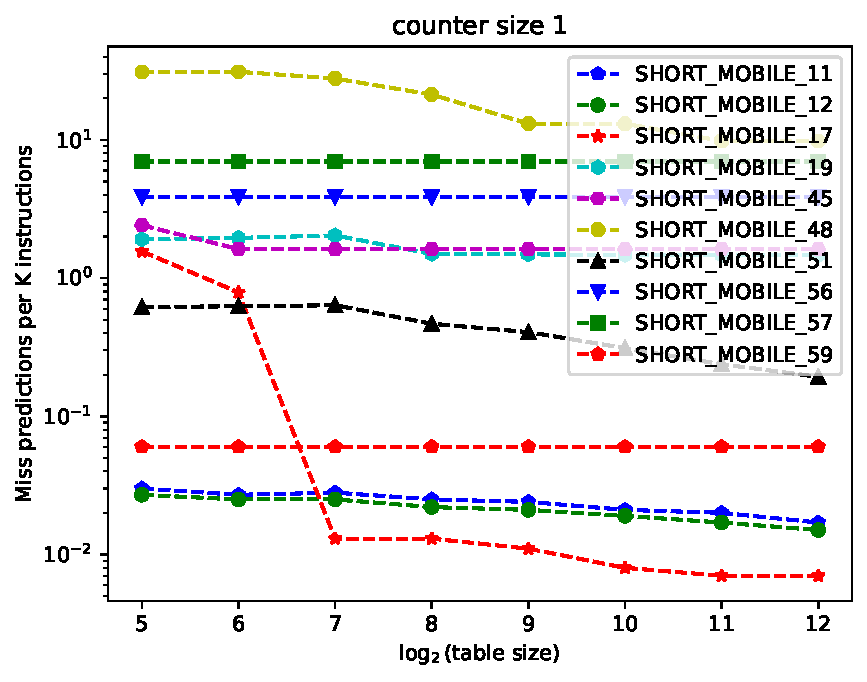
\includegraphics[width=\linewidth]{default-predictor/graph_1}
\end{minipage}%
\hfill
\begin{minipage}{.48\linewidth}
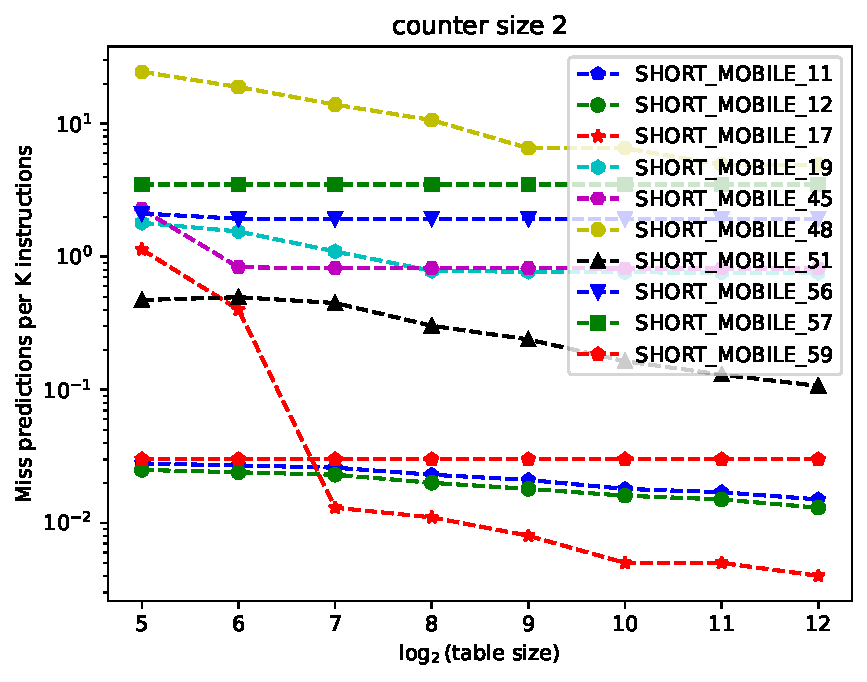
\includegraphics[width=\linewidth]{default-predictor/graph_2}
\end{minipage}

\begin{minipage}{.48\linewidth}
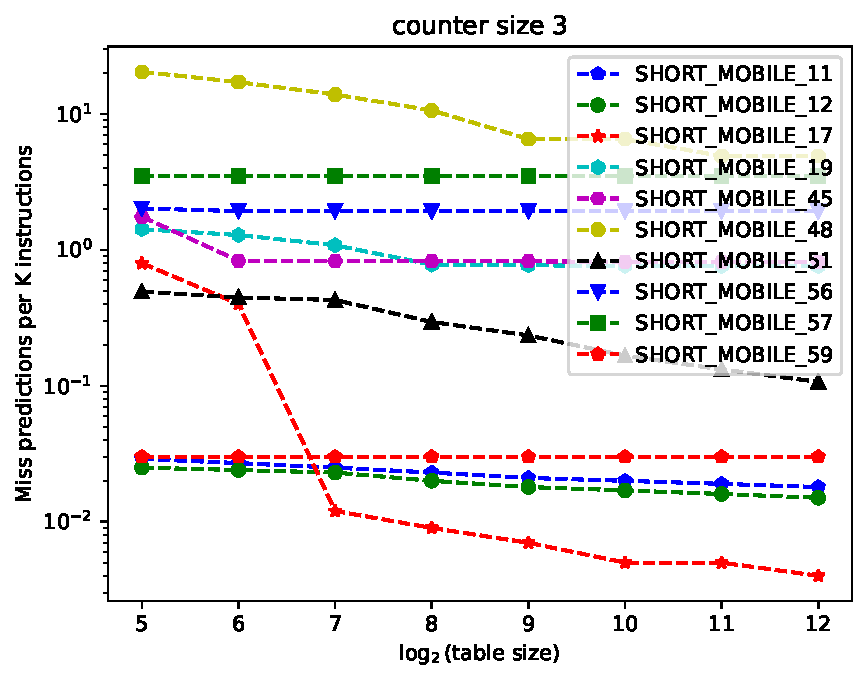
\includegraphics[width=\linewidth]{default-predictor/graph_3}
\end{minipage}%
\hfill
\begin{minipage}{.48\linewidth}
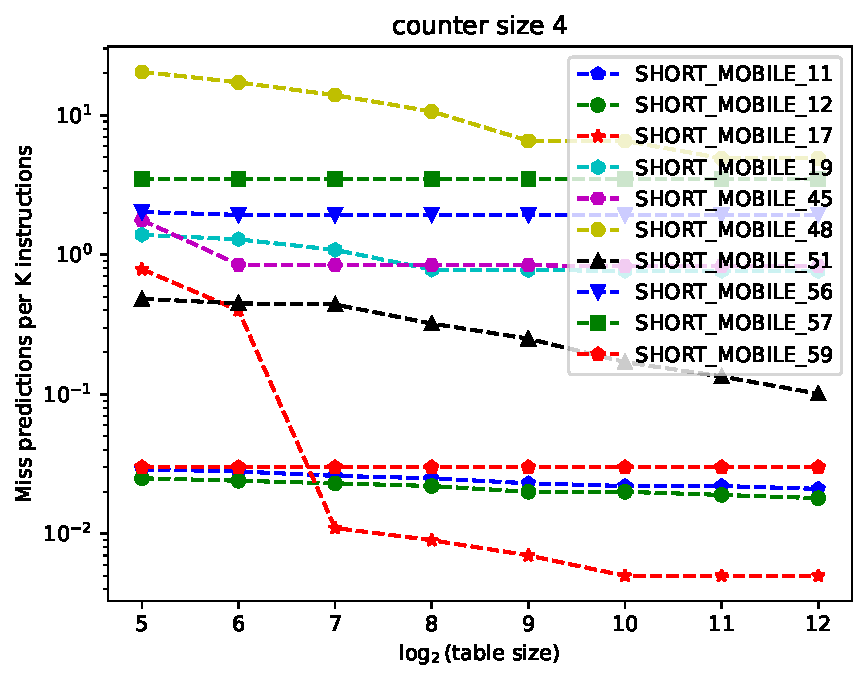
\includegraphics[width=\linewidth]{default-predictor/graph_4}
\end{minipage}

\begin{minipage}{.48\linewidth}
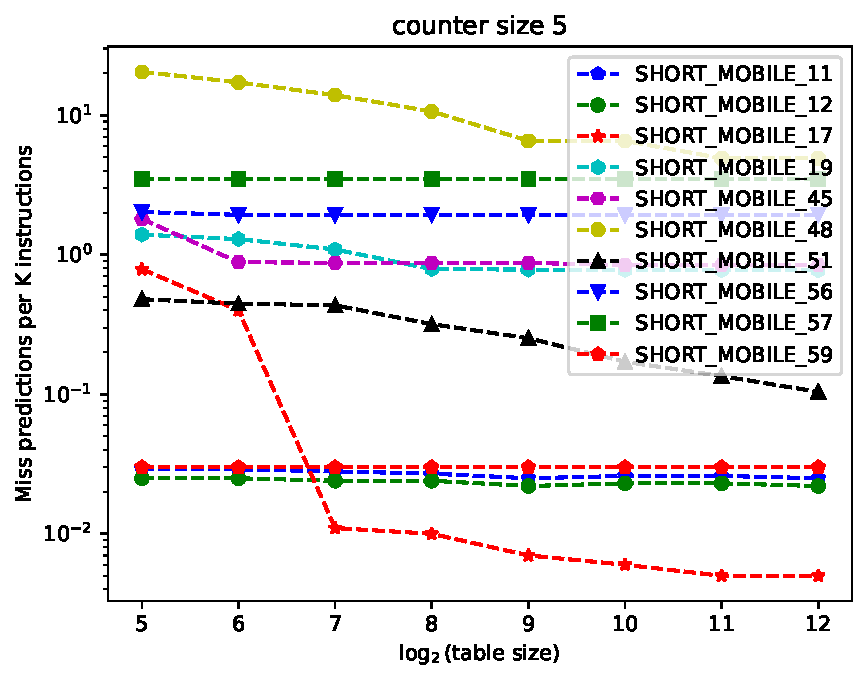
\includegraphics[width=\linewidth]{default-predictor/graph_5}
\end{minipage}%
\hfill
\begin{minipage}{.48\linewidth}
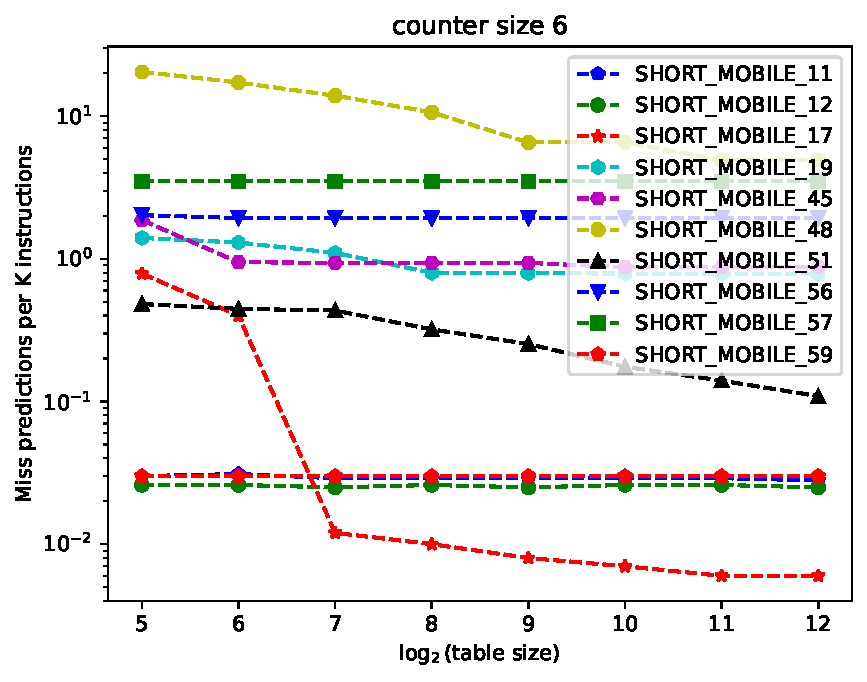
\includegraphics[width=\linewidth]{default-predictor/graph_6}
\end{minipage}
\subsection{Analyse}
On voit une asymptote due à la disparition des collisions lorsque la taille du prédicteur augmente.
Le coût du prédicteur est linéaire avec la taille du tableau, et il n'est pas raisonnable de dépasser $2^{16}$ éléments, d'autant que le gain à partir de $2^{12}$ devient très faible.
Par ailleurs, il y a toujours moins de $7\%$ de mauvaise prédictions, ce qui est remarquable pour une approche aussi simpliste.


Nous remarquons aussi que les gains pour un \textit{counter size} supérieure à 2 sont négligeables. En ce qui concerne la taille de la table, nous remarquons qu'à partir de 10, on commence à voir une asymptote pour les test 17 mais pour des autres test cette asymptote apparaît beaucoup plus tôt (11,12,57...)

\section{G Share}
\subsection{Conception}
On applique le même principe que celui utilisé pour le prédicteur $n$ modal, en incorporant un historique global. Qu'on utilise ensuite pour faire un \textit{xor} avec les bits du PC et indexer la table des compteur à états.
\subsection{Résultats}
\begin{minipage}{.48\linewidth}
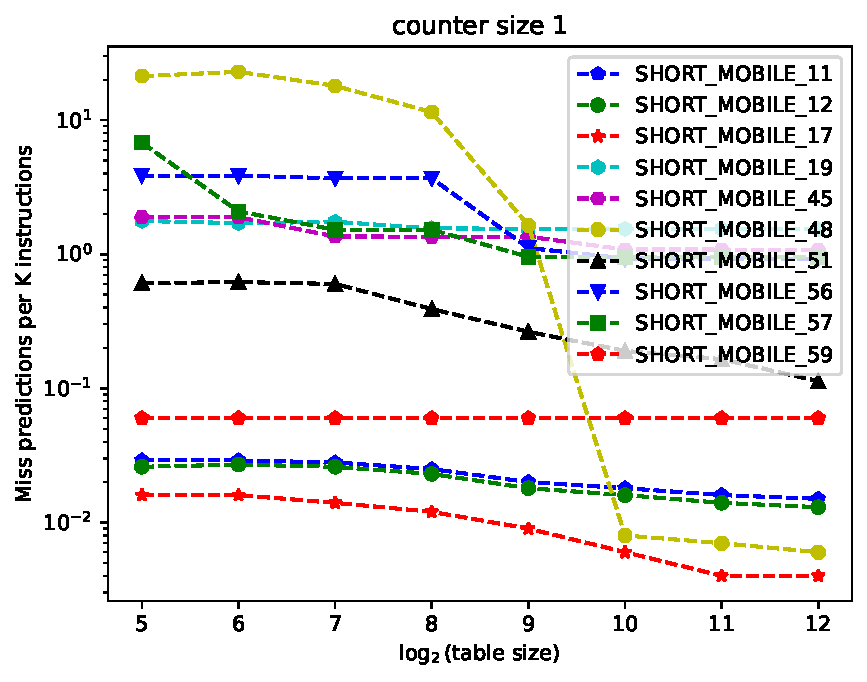
\includegraphics[width=\linewidth]{gshare/graph_1}
\end{minipage}%
\hfill
\begin{minipage}{.48\linewidth}
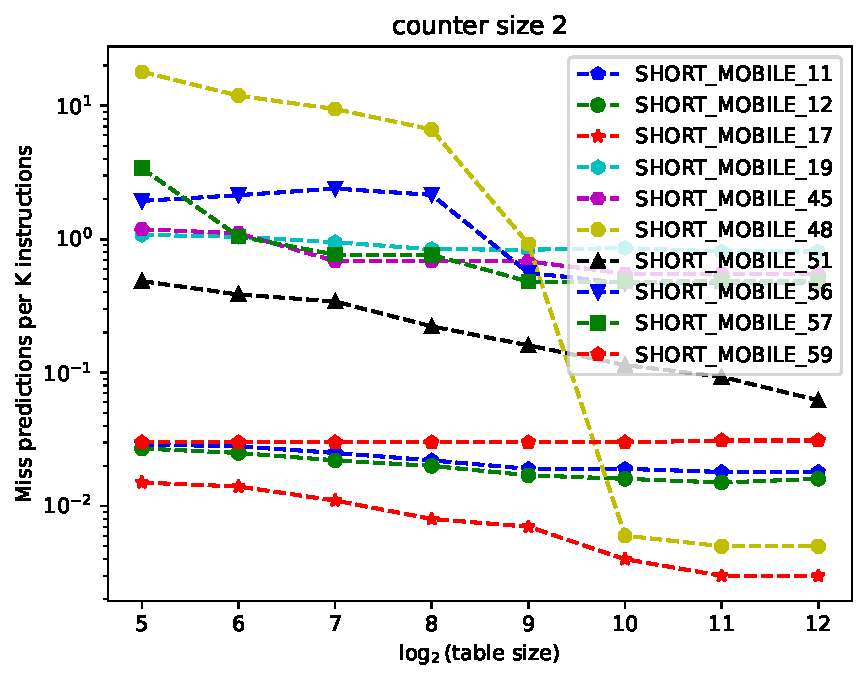
\includegraphics[width=\linewidth]{gshare/graph_2}
\end{minipage}

\begin{minipage}{.48\linewidth}
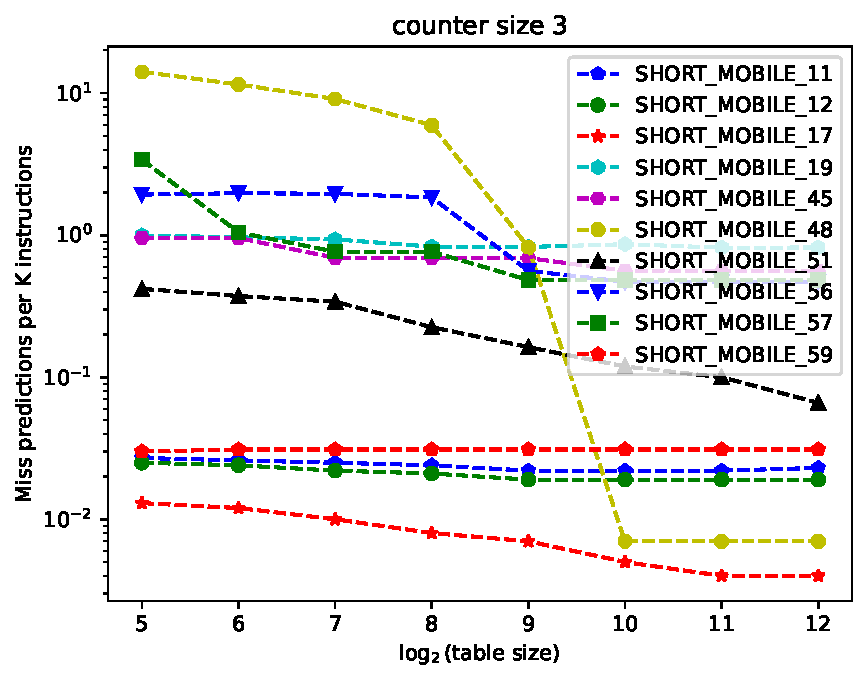
\includegraphics[width=\linewidth]{gshare/graph_3}
\end{minipage}%
\hfill
\begin{minipage}{.48\linewidth}
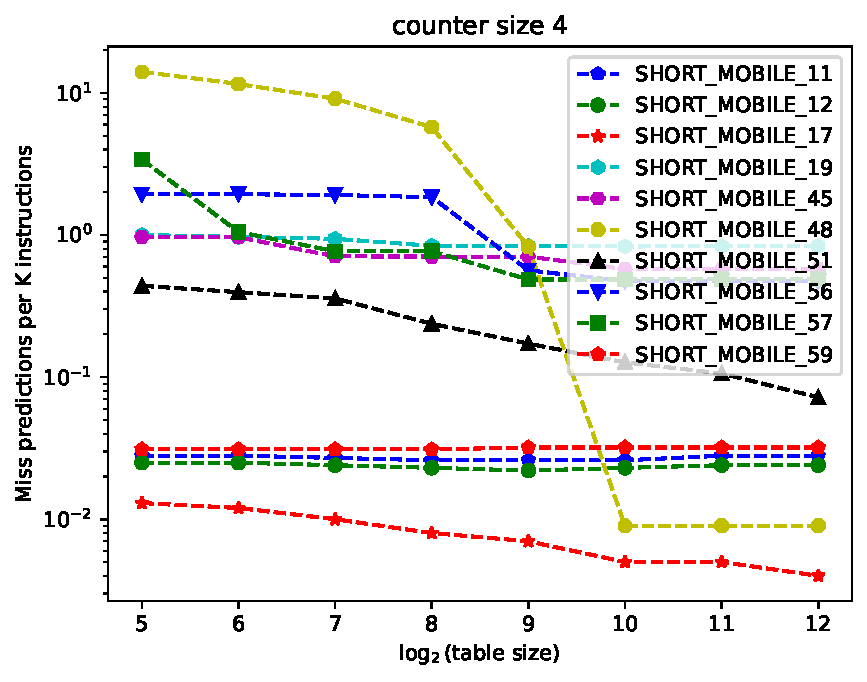
\includegraphics[width=\linewidth]{gshare/graph_4}
\end{minipage}

\begin{minipage}{.48\linewidth}
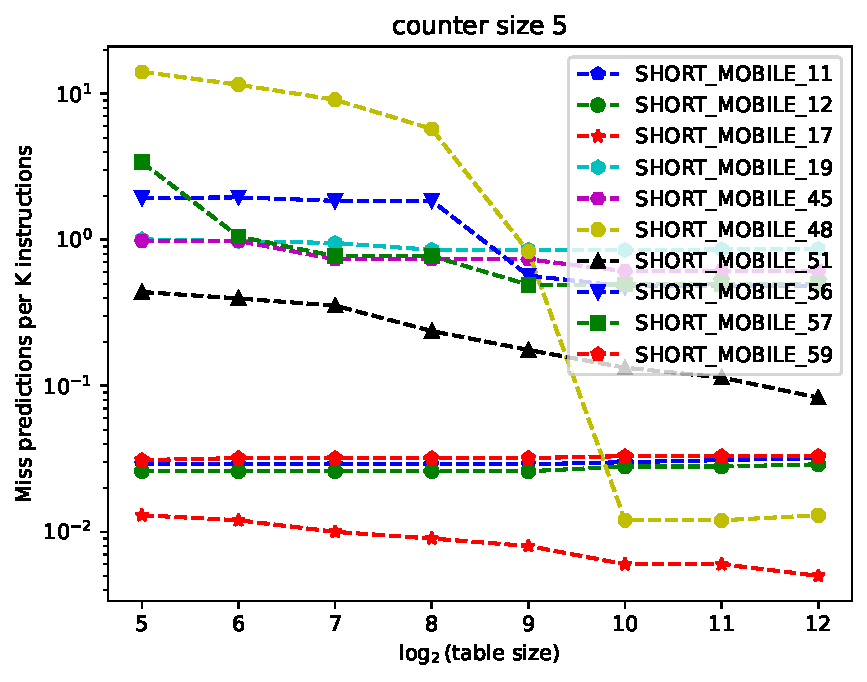
\includegraphics[width=\linewidth]{gshare/graph_5}
\end{minipage}%
\hfill
\begin{minipage}{.48\linewidth}
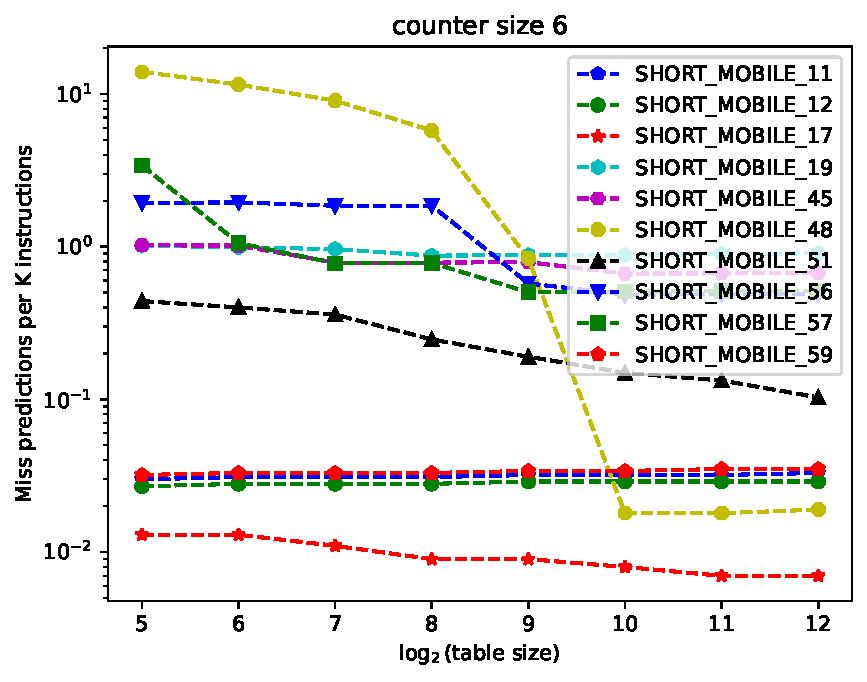
\includegraphics[width=\linewidth]{gshare/graph_6}
\end{minipage}

\subsection{Analyse}
Comme pour le prédicteur précédent, pour une taille de compteur supérieure à 2 bits, les gains sont très faibles et commencent même à être pires, donc la taille idéale semble être 2. Nous observons également une asymptote pour le test 17 à partir d'une \textit{table size} de $2^{10}$.

En comparant avec le prédicteur précédent, nous notons que ce prédicteur, pour certains tests comme le 48, parvient à obtenir des performances bien meilleures tout en maintenant les mêmes performances sur les autres tests.

\section{Predictor PHT}
\subsection{Conception}
On utilise une table d'historiques (\textit{PHT}) au lieu d'un historique globale, et on fait varier la taille de celle-ci en même temps que pour la taille de la \textit{BHT}.

\begin{minipage}{.48\linewidth}
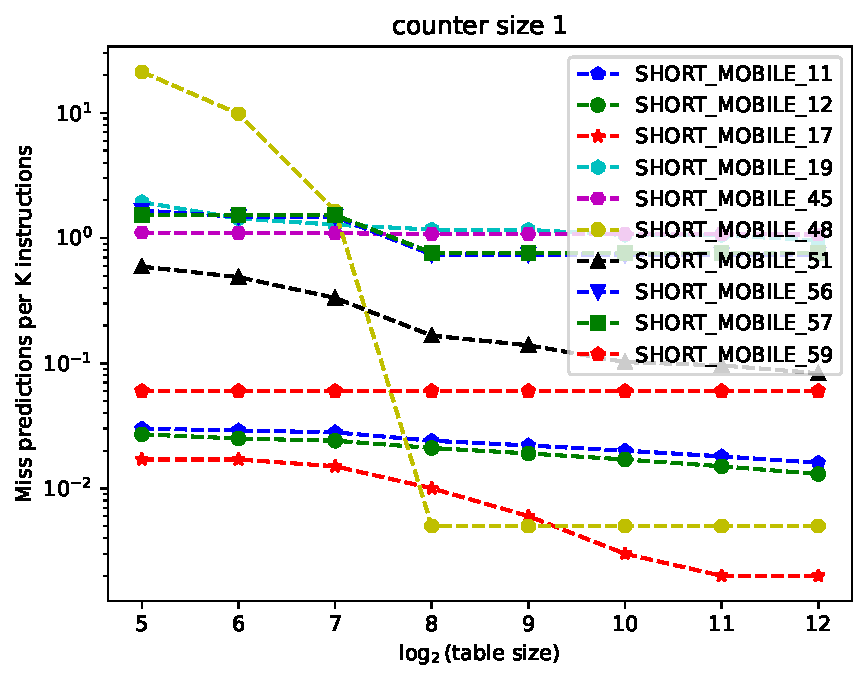
\includegraphics[width=\linewidth]{pht/graph_1}
\end{minipage}%
\hfill
\begin{minipage}{.48\linewidth}
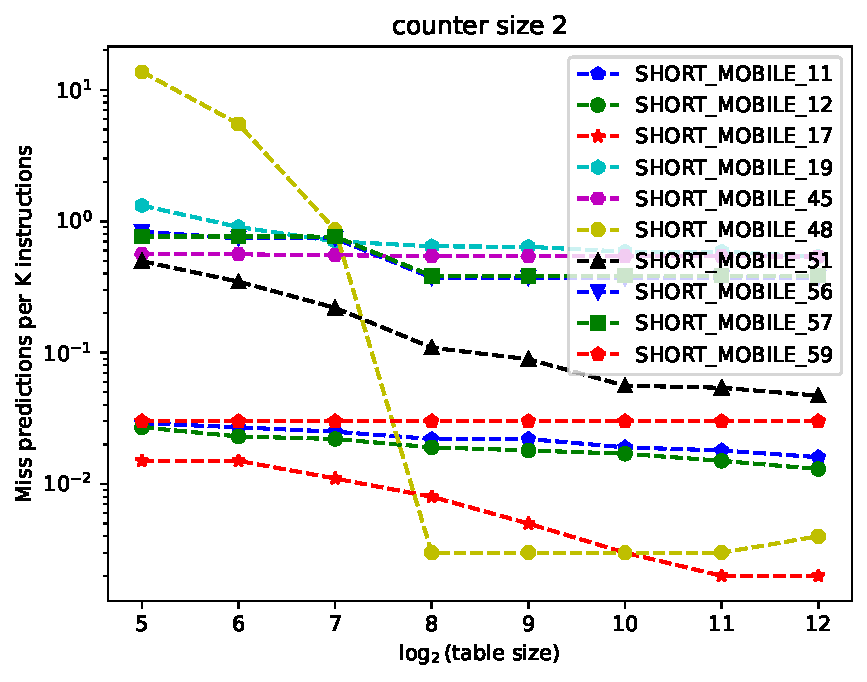
\includegraphics[width=\linewidth]{pht/graph_2}
\end{minipage}

\begin{minipage}{.48\linewidth}
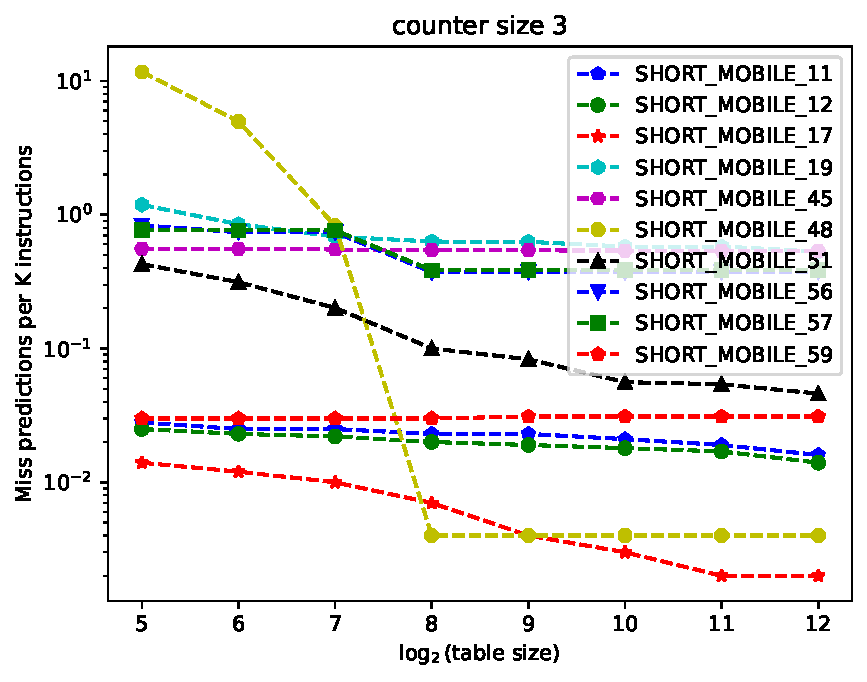
\includegraphics[width=\linewidth]{pht/graph_3}
\end{minipage}%
\hfill
\begin{minipage}{.48\linewidth}
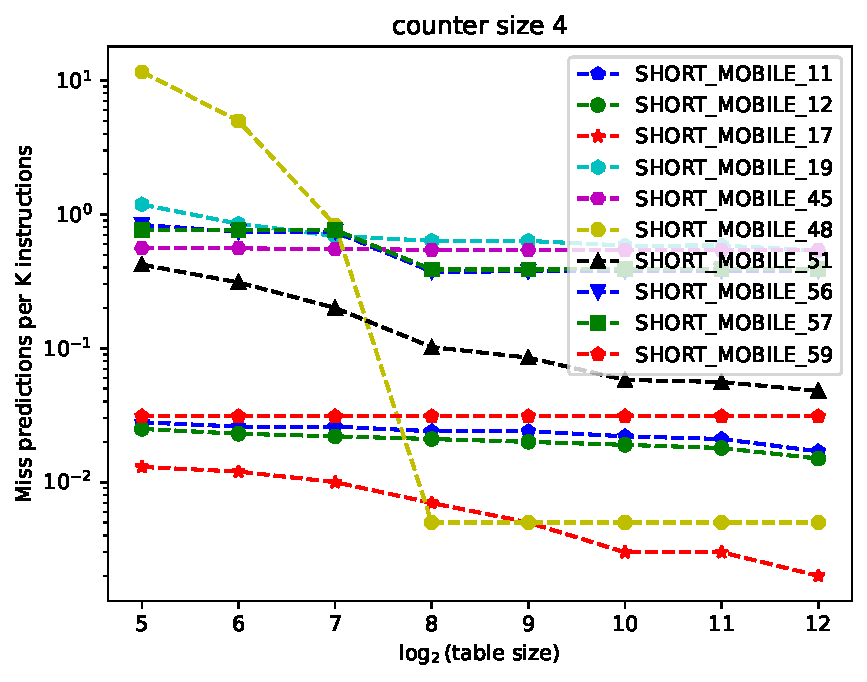
\includegraphics[width=\linewidth]{pht/graph_4}
\end{minipage}

\begin{minipage}{.48\linewidth}
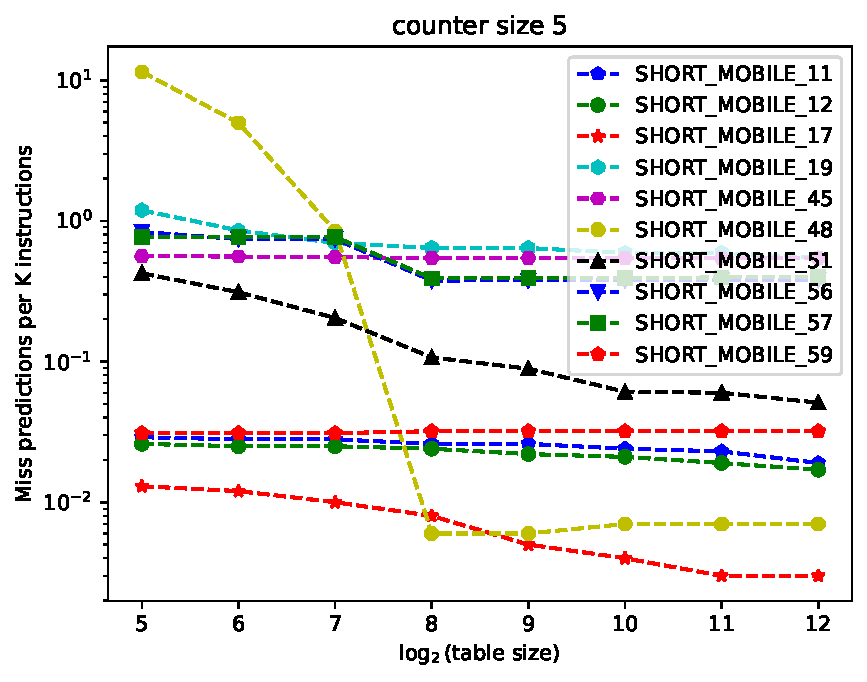
\includegraphics[width=\linewidth]{pht/graph_5}
\end{minipage}%
\hfill
\begin{minipage}{.48\linewidth}
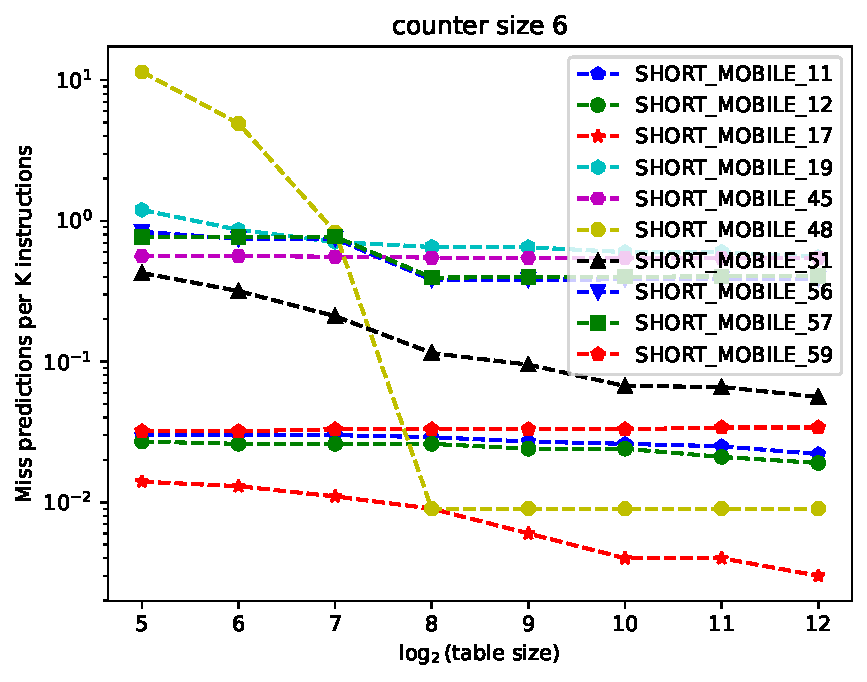
\includegraphics[width=\linewidth]{pht/graph_6}
\end{minipage}

\subsection{Analyse}

Nous remarquons que pour des tailles plus petites, notre prédicteur atteint une asymptote beaucoup plus tôt que le \textit{gshare}, surtout pour le test 48. Pour les autres tests, les gains sont peu significatifs, et à partir de 1024 entrées, le \textit{gshare} présente à peu près le même comportement que le prédicteur \textit{PHT}.


\section{Dual predictor}
\subsection{Conception}
Nous construisons les 2 prédicteurs avec les paramètres suivants : \textit{gshare} avec un historique de 1024 entrées et un tableau de compteurs à 2 bits de taille 1024 également. 
Pour la \textit{PHT}, nous utilisons 1024 entrées, et pour la \textit{BHT}, nous utilisons également 1024 entrées, indexées par des compteurs à 2 bits.

Nous décidons quel prédicteur utiliser grâce au méta-prédicteur qui est composé de 1024 entrées de compteurs bimodaux.

\subsection{Résultats}
\begin{minipage}{.48\linewidth}
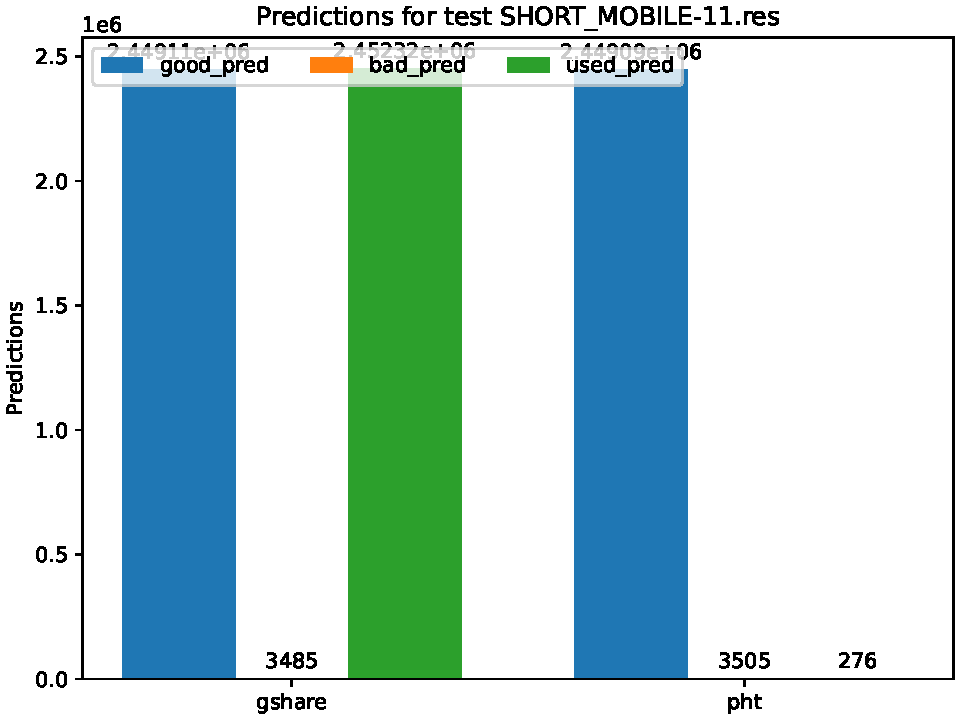
\includegraphics[width=\linewidth]{graphs/dual-predictor/preds_SHORT_MOBILE-11.res.pdf}
\end{minipage}%
\hfill
\begin{minipage}{.48\linewidth}
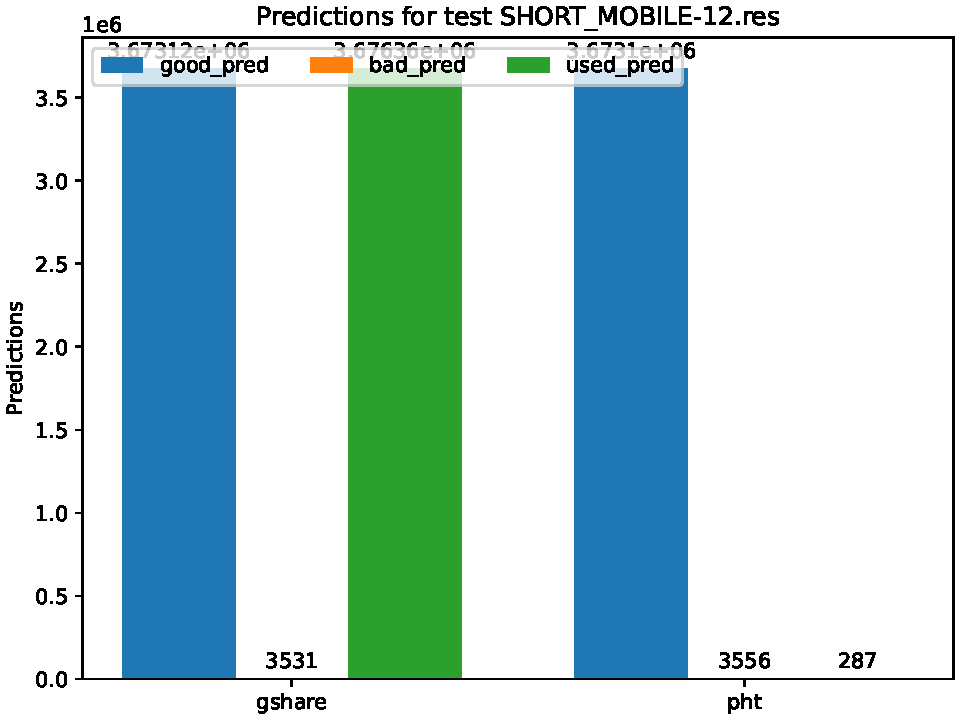
\includegraphics[width=\linewidth]{graphs/dual-predictor/preds_SHORT_MOBILE-12.res.pdf}
\end{minipage}

\begin{minipage}{.48\linewidth}
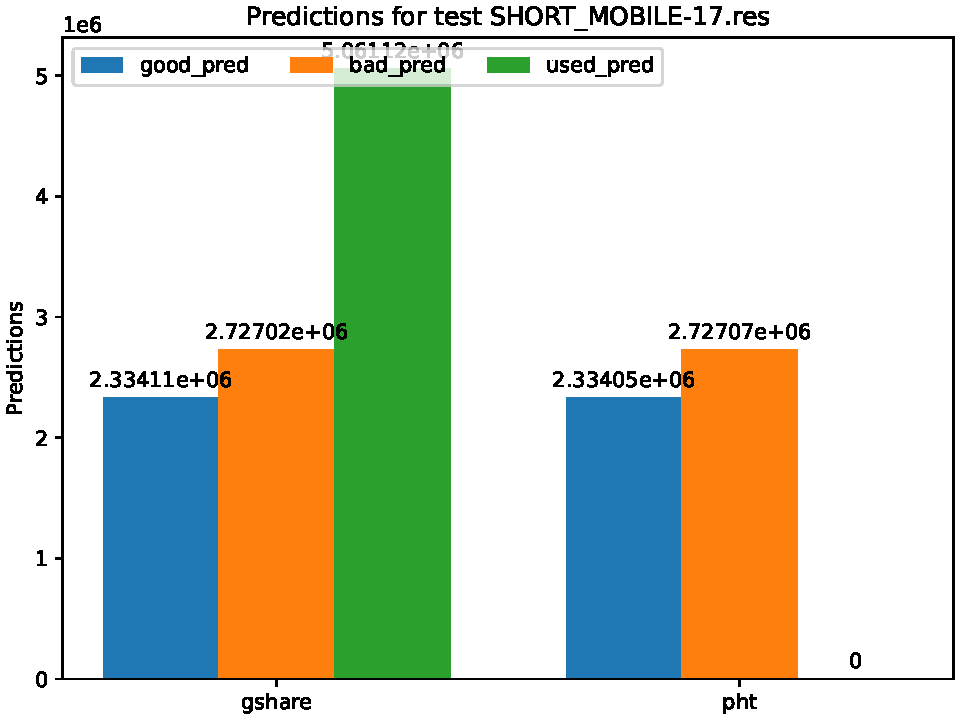
\includegraphics[width=\linewidth]{graphs/dual-predictor/preds_SHORT_MOBILE-17.res.pdf}
\end{minipage}%
\hfill
\begin{minipage}{.48\linewidth}
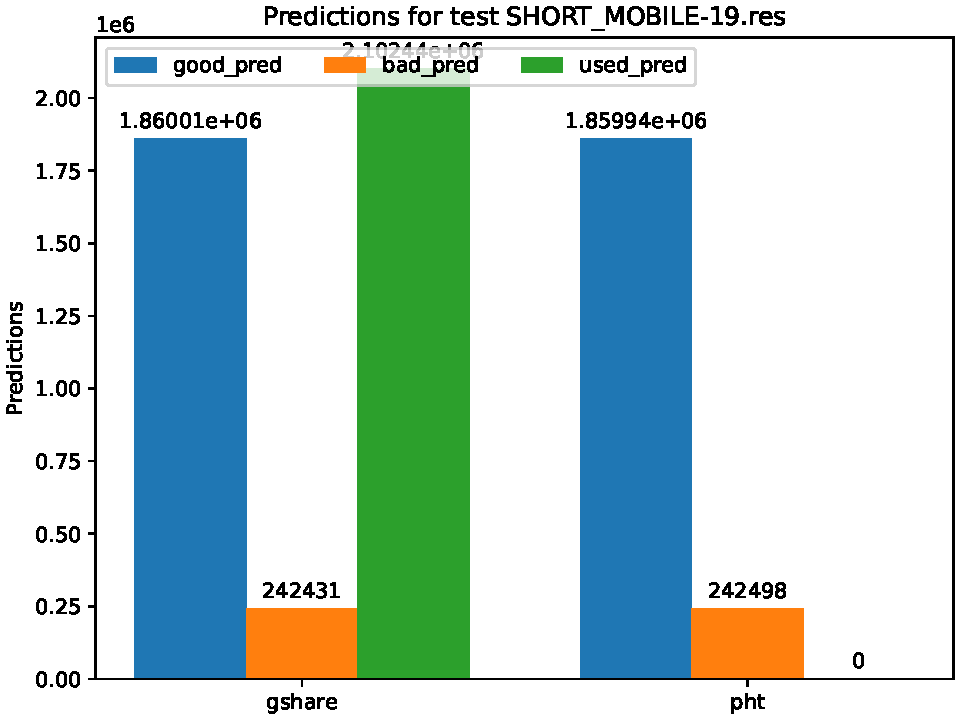
\includegraphics[width=\linewidth]{graphs/dual-predictor/preds_SHORT_MOBILE-19.res.pdf}
\end{minipage}

\begin{minipage}{.48\linewidth}
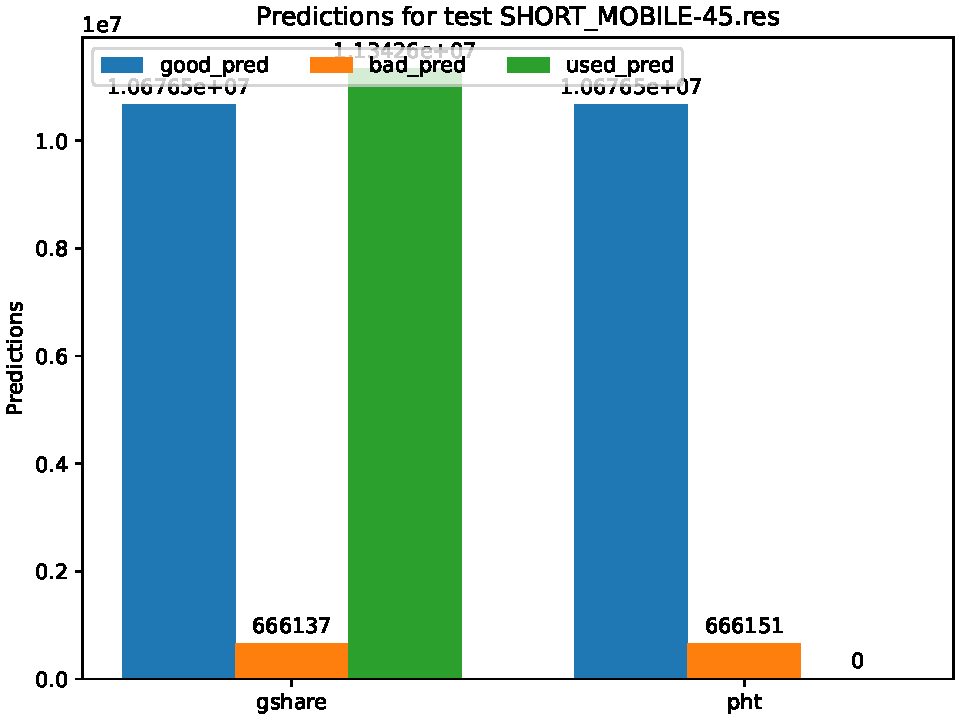
\includegraphics[width=\linewidth]{graphs/dual-predictor/preds_SHORT_MOBILE-45.res.pdf}
\end{minipage}%
\hfill
\begin{minipage}{.48\linewidth}
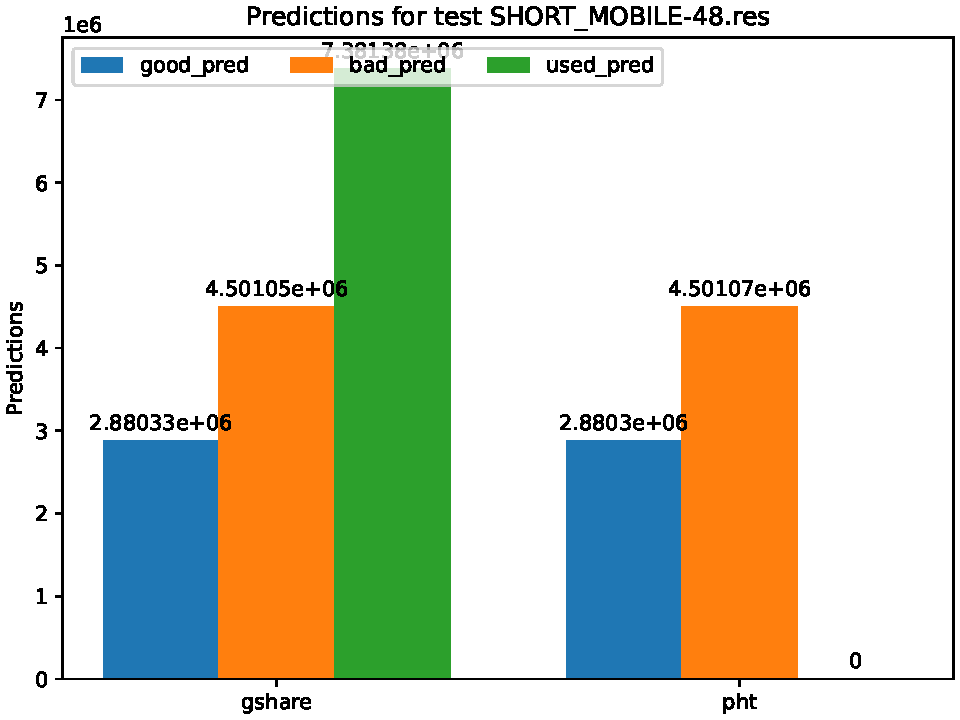
\includegraphics[width=\linewidth]{graphs/dual-predictor/preds_SHORT_MOBILE-48.res.pdf}
\end{minipage}

\begin{minipage}{.48\linewidth}
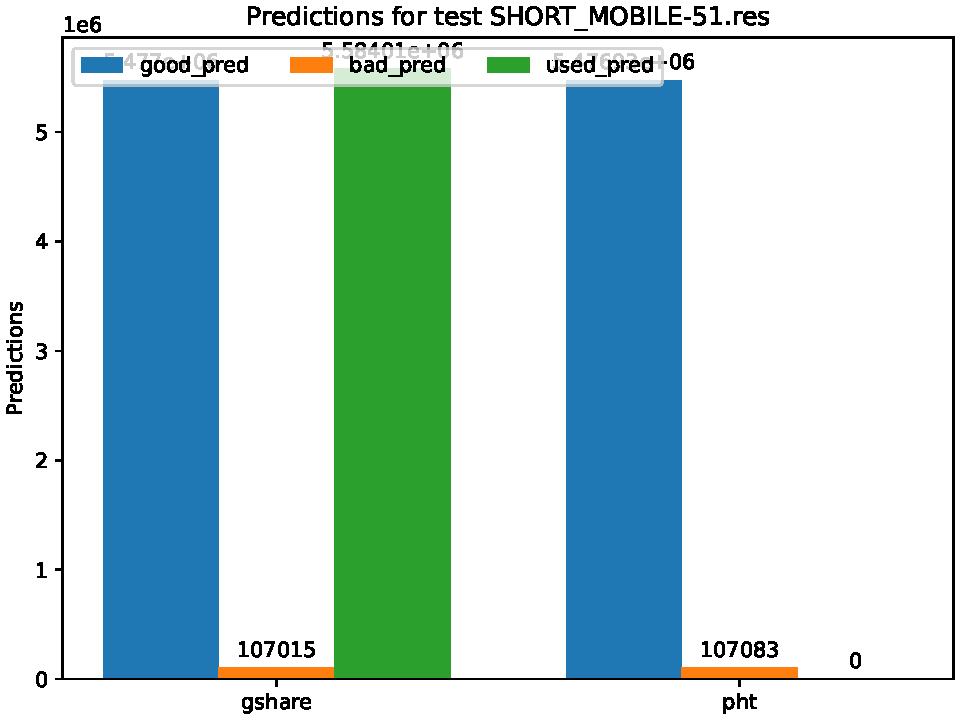
\includegraphics[width=\linewidth]{graphs/dual-predictor/preds_SHORT_MOBILE-51.res.pdf}
\end{minipage}%
\hfill
\begin{minipage}{.48\linewidth}
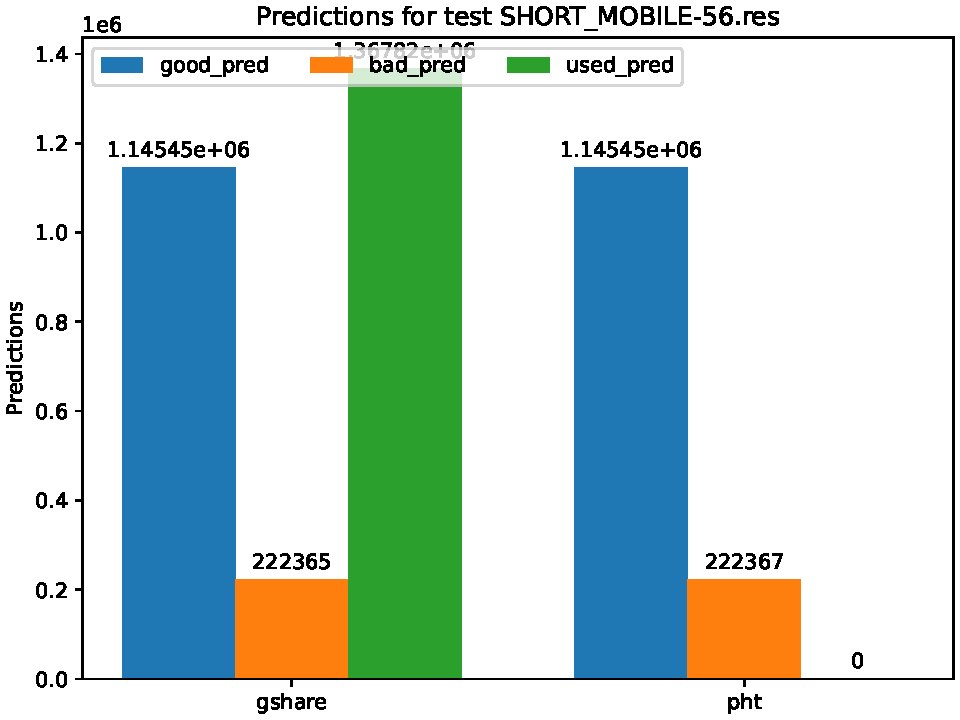
\includegraphics[width=\linewidth]{graphs/dual-predictor/preds_SHORT_MOBILE-56.res.pdf}
\end{minipage}

\begin{minipage}{.48\linewidth}
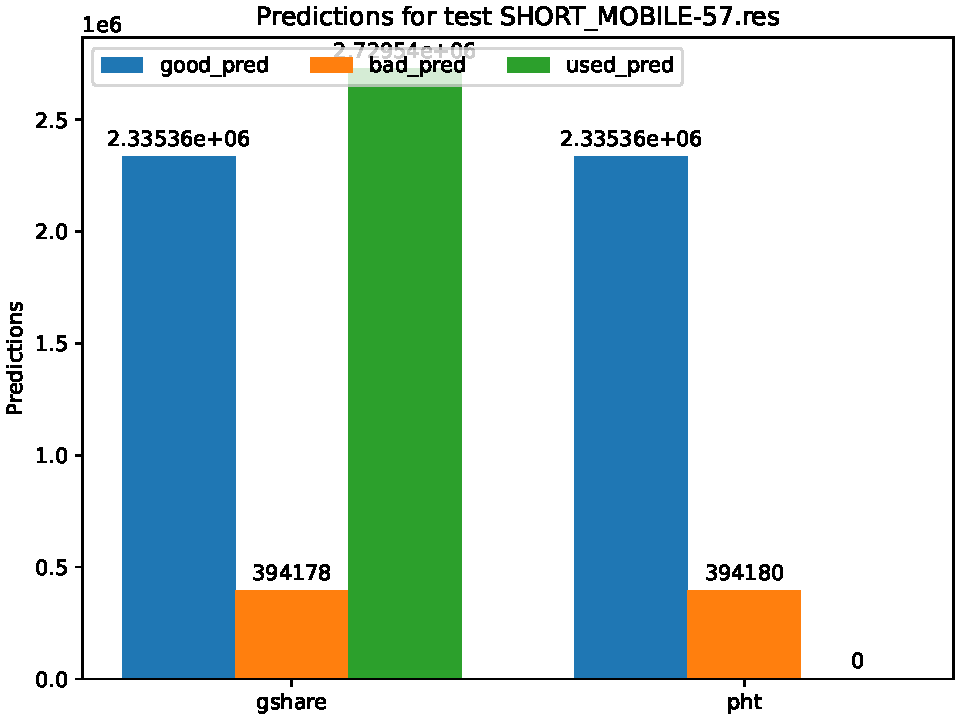
\includegraphics[width=\linewidth]{graphs/dual-predictor/preds_SHORT_MOBILE-57.res.pdf}
\end{minipage}%
\hfill
\begin{minipage}{.48\linewidth}
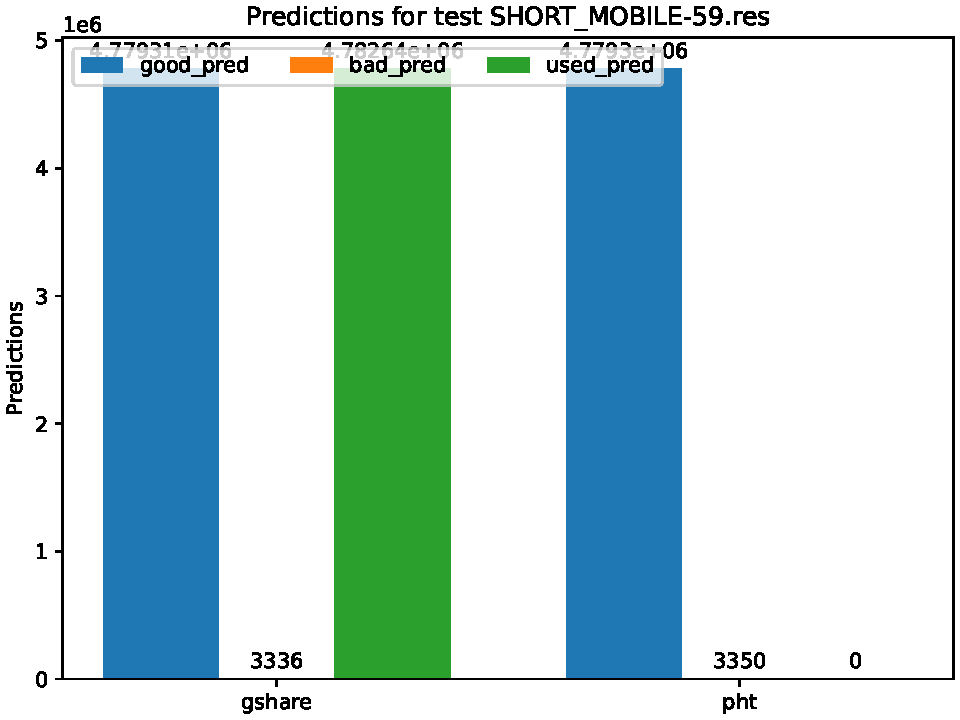
\includegraphics[width=\linewidth]{graphs/dual-predictor/preds_SHORT_MOBILE-59.res.pdf}
\end{minipage}

\subsection{Analyse}

Nous observons un comportement très similaire des deux prédicteurs, ce qui est cohérent avec les résultats précédents. Si nous examinons les graphiques précédents pour une \textit{counter size} de deux et une \textit{table size} de 10, les résultats sont presque identiques. Il aurait été intéressant d'analyser les différences pour des tableaux de taille $2^8$, car nous aurions pu constater une amélioration des performances du prédicteur \textit{PHT} par rapport au \textit{gshare}.

\section{Perceptron}
\subsection{Conception}
Les \textit{counter size} dans la section suivante représentent des valeurs de $ \theta * 5 $. Par exemple, une \textit{counter size} de 5 représente un $\theta$ de 25.
\subsection{Résultats}
\begin{minipage}{.48\linewidth}
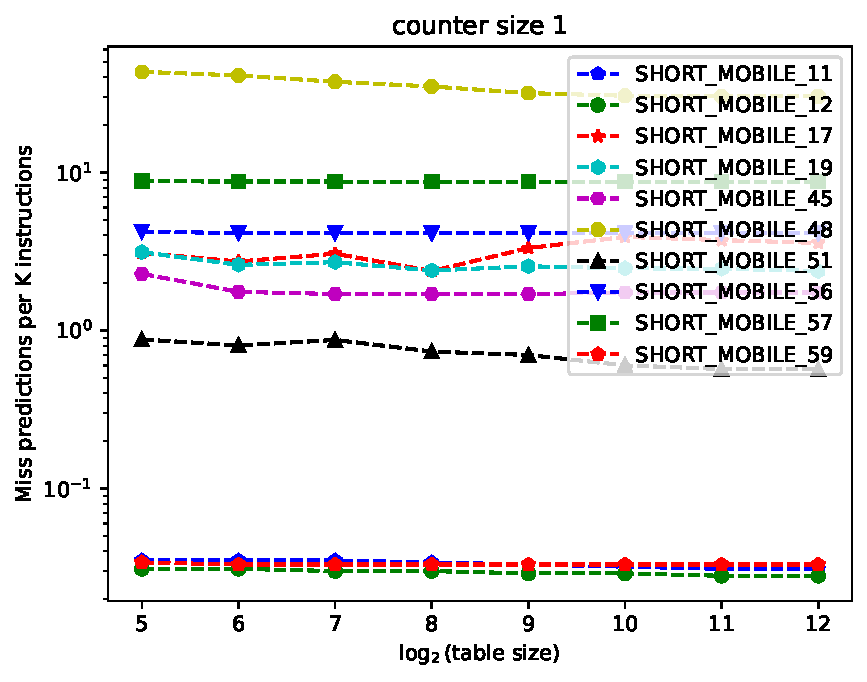
\includegraphics[width=\linewidth]{perceptron/graph_1}
\end{minipage}%
\hfill
\begin{minipage}{.48\linewidth}
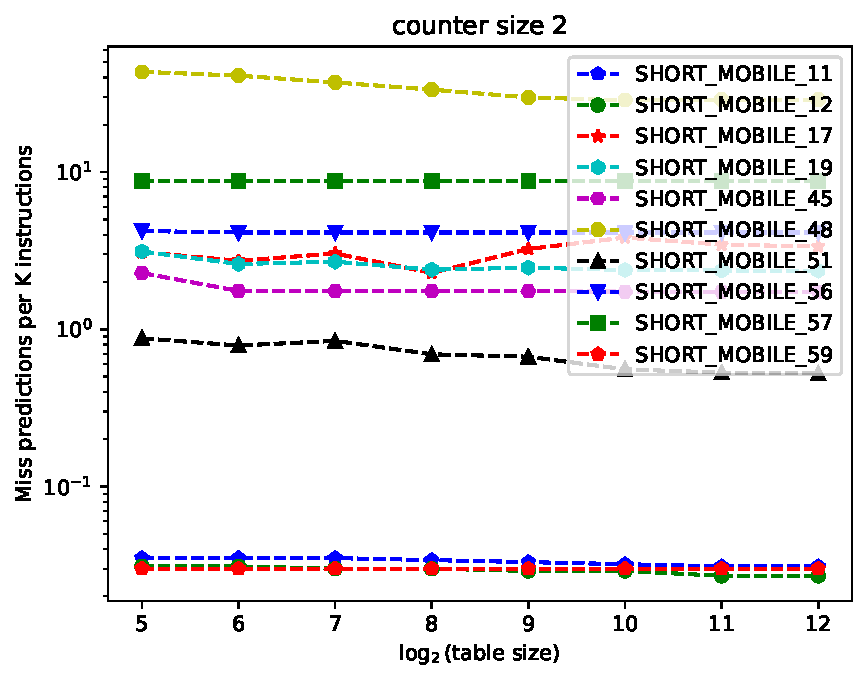
\includegraphics[width=\linewidth]{perceptron/graph_2}
\end{minipage}

\begin{minipage}{.48\linewidth}
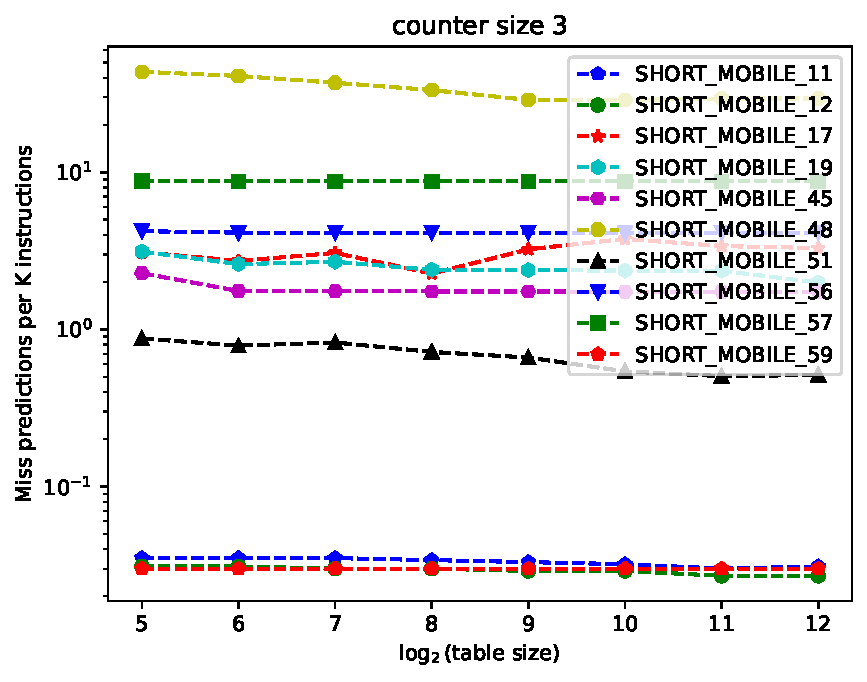
\includegraphics[width=\linewidth]{perceptron/graph_3}
\end{minipage}%
\hfill
\begin{minipage}{.48\linewidth}
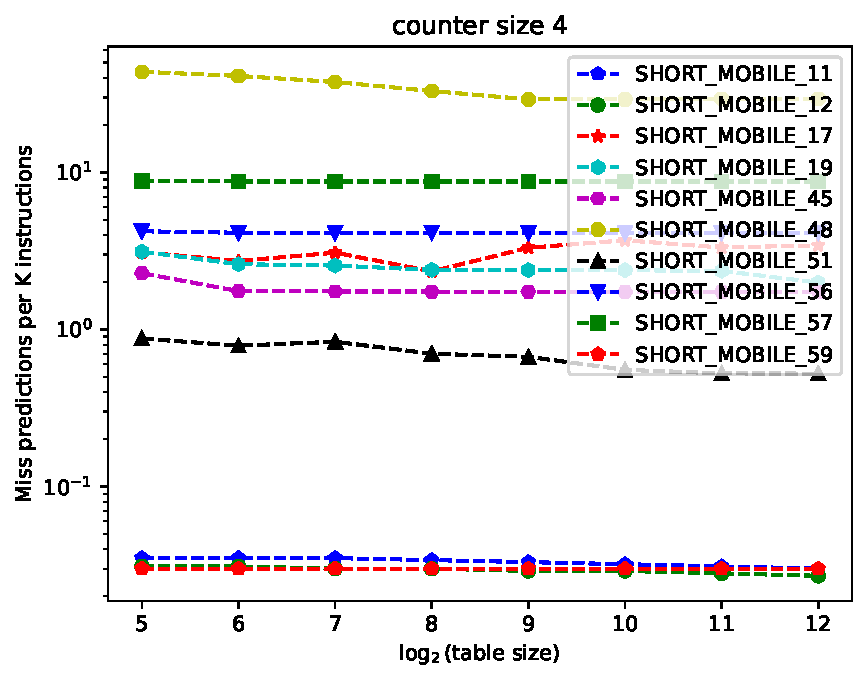
\includegraphics[width=\linewidth]{perceptron/graph_4}
\end{minipage}

\begin{minipage}{.48\linewidth}
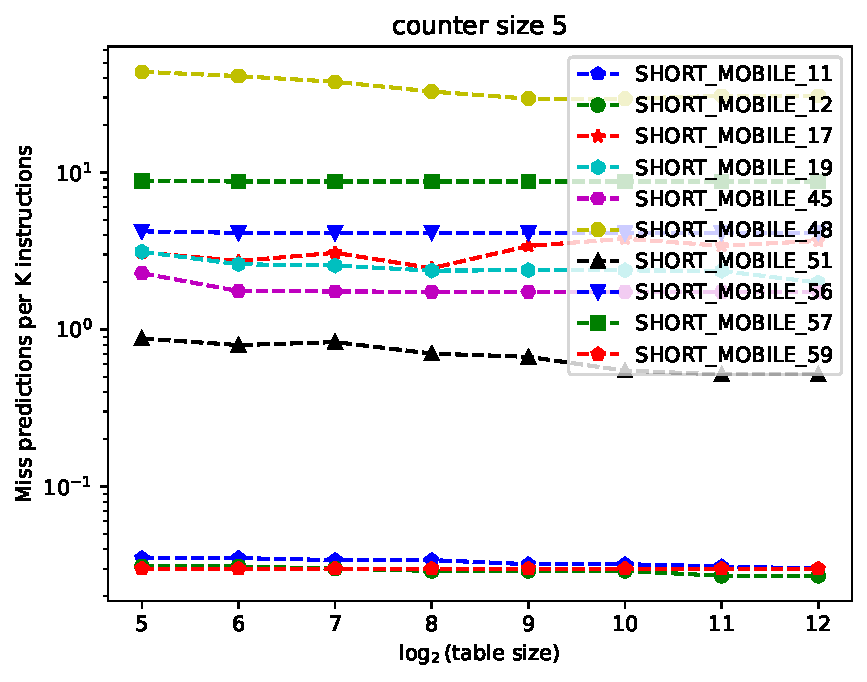
\includegraphics[width=\linewidth]{perceptron/graph_5}
\end{minipage}%
\hfill
\begin{minipage}{.48\linewidth}
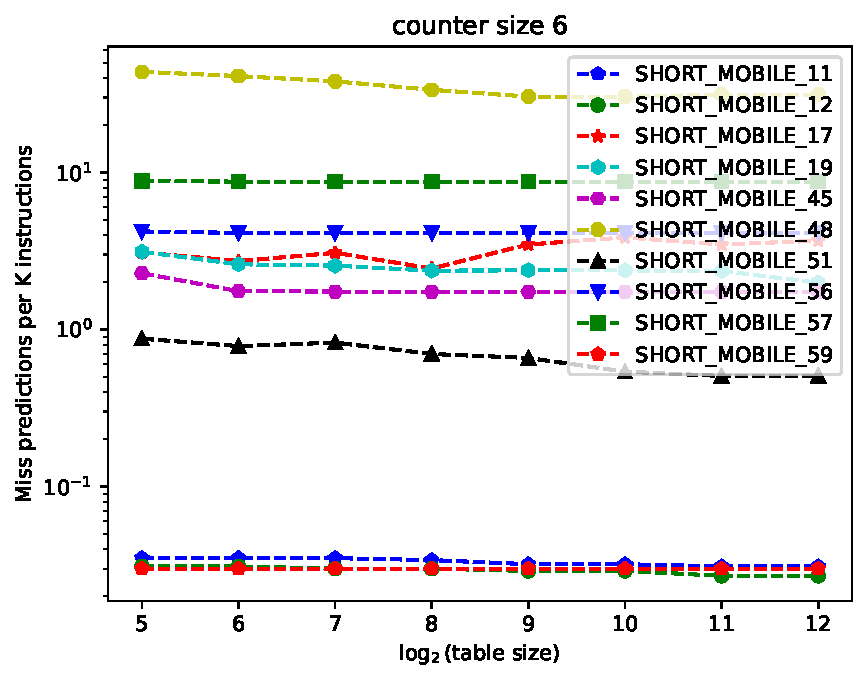
\includegraphics[width=\linewidth]{perceptron/graph_6}
\end{minipage}
\subsection{Analyse}
Les performances du prédicteur perceptron sont assez décevantes, ne surpassant pas le \textit{gshare} et ajoutant une complexité supplémentaire avec le calcul de $y$.
\end{document}
